\documentclass[9pt,twoside]{pnas-new}
% Use the lineno option to display guide line numbers if required.

\templatetype{pnassupportinginfo}
%\readytosubmit %  % Uncomment this line before submitting, so that the instruction page is removed.

\title{Weber-Fechner gain control enhances the fidelity of combinatorial odor coding}
\author{Nirag Kadakia and Thierry Emonet}
\correspondingauthor{Nirag Kadakia.\\E-mail: nirag.kadakia@yale.edu}

\begin{document}

%% Comment/remove this line before generating final copy for submission
%\instructionspage  

%\maketitle

%% Adds the main heading for the SI text. Comment out this line if you do not have any supporting information text.
\SItext

\section*{Mathematical model}

\subsection*{Model of odor binding, Or/Orco activation, and ORN firing}

We model an odor as an $N$-dimensional vector ${\mathbf s=[ s_1,...,s_N]}$, where $s_i > 0$ are the concentrations of individual volatile molecules (odorants) comprising the odor. 
The olfactory sensory system is modeled as a collection of $M$ distinct Or/Orco complexes indexed by the sub index $a=1,...,M$, each of which can be bound with any one of the odorant molecules, and can be either active (firing) or inactive (quiescent). At first we assume there is one binding site per complex; this will be generalized to many sites. We consider the binding and activation processes to be in equilibrium, assigning each state a corresponding Boltzmann weight, where the zero of energy is set by the unbound, inactive state $C_a$. These weights are:
\begin{align}
    &C_a        &&      1 \nonumber \\
    &C^*_a      &&      \exp({-\beta \epsilon_a}) \nonumber \\
    &C_as_i     &&      \exp({-\beta(-E_{ai}  - \mu_{i})}) \nonumber \\
    &C^*_as_i   &&      \exp({-\beta(-(E_{ai}^* - \epsilon_a) - \mu_{i}}),
\end{align}
where $\epsilon_a$ (assumed positive) is the free energy difference between the active and inactive conformation of the unbound receptor, and $E_{ai}$ and $E_{ai}^*$ are the free energy differences (assumed positive) between the unbound and bound state for the inactive and active receptor, respectively. $\mu_{i}=\mu_0+\beta^{-1}\log(s_i/s_0)$ is the chemical potential for odorant species $i$ in terms of a reference chemical potential $\mu_0$ at concentration $s_0$, $s_0\exp(-\beta \mu_0) = s_i\exp(-\beta \mu_{i})$, which can be traded for the thermodynamic-relevant disassociation constants $K_{ai} = s_0 e^{\beta (-E_{ai} - \mu_0)}$. %In terms of thermodynamic quantities, the Boltzmann weights therefore read:
%\begin{align}
%    &C_a        &&      1 \nonumber \\
%    &C^*_a      &&      \exp({-\beta \epsilon_a}) \nonumber \\
%    &C_as_i     &&      \frac{s_i}{K_{ai}} \nonumber \\
%    &C^*_as_i   &&      \exp({-\beta %\epsilon_a})\frac{s_i}{K^*_{ai}},
%\end{align}
Adding up contributions from all $i$ odorants, the active fraction is:
\begin{align}
A_a &= \frac{
    C^*_a + \sum_i C^*_as_i}{C_a + \sum_i C_as_i + C^*_a + \sum_i C^*_as_i} %\nonumber 
    = 
    \left(1 + e^{\epsilon_a}\frac{1 + \sum_i^N \frac{s_i}{K_{ai}}}{1 + \sum_i^N \frac{s_i}{K^*_{ai}}}
    \right)^{-1}, 
    \label{eq:steady_state_act}
\end{align} 
where we have expressed free energies in units of $k_B T=\beta^{-1}$ for notational convenience.

This expression can be generalized for the case of multiple, independent binding sites through some simple combinatorial factors. Consider first an odorant $i$ which can bind one of two locations on receptor $a$. There are then 4 possible inactive states: both sites unbound, site 1 bound, site 2 bound, both sites bound. Combined with the active states, there are therefore 8 states for odorant $i$ and receptor $a$, with energies: 
\begin{align}
& \textup{active}  && \{1, \quad -E_{ai} - \mu_i, \quad -E_{ai} - \mu_i, \quad -2E_{ai} - 2\mu_i\} \nonumber \\
& \textup{inactive}  && \{\epsilon_a, \quad -(E^*_{ai}  - \epsilon_a) - \mu_i, \quad -(E^*_{ai}  - \epsilon_a) - \mu_i, \quad -(2E^*_{ai}  - \epsilon_a) - 2\mu_i\} 
\end{align}
In the active fraction, Eq.~\ref{eq:steady_state_act}, the Boltzmann factors combine through the binomial theorem, giving (for a single odorant environment $i$):
\begin{align}
A_a(\textup {odorant }i \textup{, 2 binding sites}) &= 
    \left(1 + e^{\epsilon_a}\frac{(1 + \frac{s_i}{K_{ai}})^2}{(1 + \frac{s_i}{K^*_{ai}})^2}
    \right)^{-1}.
\end{align} 
This expression generalizes for an arbitrary number of odorants and independent binding sites through the appropriate combinatorial factors, giving an active fraction of
\begin{align}
A_a(N \textup { odorants}, R \textup { binding sites}) &= 
    \left[1 + e^{\epsilon_a}\left(\frac{1 + \sum_i^N\frac{s_i}{K_{ai}}}{1 + \sum_i^N \frac{s_i}{K^*_{ai}}}\right)^R\right]^{-1}. 
\end{align} 
Finally, firing rate dynamics are assumed linear-nonlinear:
\begin{align}
r_a(t) &= f\left(\int^t h(t - \tau) A(\tau) d\tau\right) \label{eq:firing_machinery},
\end{align}
where $h(t)$ and $f$ are a temporal filter and rectifying linear unit (with threshold $\theta$ = 5 Hz) as noted in the main text.





%%%% BELOW REMOVED



\iffalse

Consider the case of 2 odorants $i$ and $j$ and 3 independent binding sites on receptor $a$ (we suppress the receptor index for now). There are $3^3$ = 27 inactive states: each binding site can be empty, occupied with $i$ or occupied with $j$. Denote the total number of $i$ and $j$ bound as a 2-tuple $(..,..)$, so for example one $i$ and two $j$ bound is (1, 2). The 27 inactive states break into:
\begin{align}
    &\textup{state} && \textup{multiplicity} &&& \textup{energy} \nonumber \\
    &(0, 0)         && 1                     &&&  0 \nonumber \\
    &(1, 0)         && 3                     &&&  E_i \nonumber \\
    &(0, 1)         && 3                     &&&  E_j \nonumber \\
    &(1, 1)         && 6                     &&&  E_i + E_j \nonumber \\
    &(2, 0)         && 3                     &&&  2E_i \nonumber \\
    &(0, 2)         && 3                     &&&  2E_j \nonumber \\
    &(2, 1)         && 3                     &&&  2E_i + E_j \nonumber \\
    &(1, 2)         && 3                     &&&  E_i + 2E_j \nonumber \\
    &(3, 0)         && 1                     &&&  3E_i \nonumber \\
    &(0, 3)         && 1                     &&&  3E_j \nonumber,
\end{align}
where $E_i = E_{ai} + \mu_i$ and $E_j = E_{aj} + \mu_j$ and, analogously for the 27 inactive states, except each energy also includes $+\epsilon_a$. The sum of the inactive Boltzmann weights factors into $(1 + \exp(-E_i) + \exp(-E_j))^3$. This generalizes to $N$ odorants with $R$ binding sites as $(1 + \sum_i^N \exp(-E_i))^R$, producing an active fraction:

\fi


%%%% ABOVE REMOVED






%%% BELOW REMOVED %%% 




\iffalse

With $N$ possible odorants, receptor $a$ resides in one of $2(N+1)$ possible states, \{$C_a$, $C^*_a$, $C_a$-$s_i$, $C^*_a$-$s_i$\}, indicating receptors that are unbound/inactive, unbound/active, inactive/bound to odorant $i$, and active/bound to odorant $i$, respectively. We assume that odor binding and unbinding is faster than receptor activation and adaptation timescale. In this limit, the binding dynamics of the $2N + 2$ states are described by master equations:

\begin{align}
\frac{d[C_a\text{-}s_i]}{dt} &= k^+_{ai}s_i[C_a] - k^-_{ai}[C_a\text{-}s_i] \label{eq:Meq_inactive_bind_rate}\\
\frac{d[C^*_a\text{-}s_i]}{dt} &= k^{*+}_{ai}s_i[C^*_a] - k^{*-}_{ai}[C^*_a\text{-}s_i],
\label{eq:Meq_active_bind_rate}
\end{align}
when receptor $C_a$ is either inactive (Eq.~\ref{eq:Meq_inactive_bind_rate}) or active (Eq.~\ref{eq:Meq_active_bind_rate}). The corresponding disassociation constants in terms of the binding transition rates are:
\begin{align}
K_{ai} = \frac{k^-_{ai}}{k^+_{ai}} \nonumber \\
K^*_{ai} = \frac{k^{*-}_{ai}}{k^{+*}_{ai}} 
\label{eq:Kd}
\end{align}

At a slower scale, transitions between inactive and active states, in any given bound state, are described by the $2N + 1$ equations:
\begin{align}
\frac{d[C_a]}{dt} &= w^{\text{u}+}_a [C_a] - w^{\text{u}-}_a [C^*_a] \label{eq:Meq_unbound_active_rate}\\
\frac{d[C^*_a\text{-}s_i]}{dt} &=  w^{\text{b}+}_{ai} [C_a\text{-}s_i] - w^{\text{b}-}_{ai}  [C^*_a\text{-}s_i],
\label{eq:Meq_bound_active_rate}
\end{align}
when receptor $C_a$ is either unbound (Eq.~\ref{eq:Meq_unbound_active_rate}) or bound (Eq.~\ref{eq:Meq_bound_active_rate}). We relate the forward and backward activation rates through a receptor- and odorant-dependent free energy difference, defined as~\cite{srinivas_elife}:
\begin{align}
%\frac{[C^*_a]}{[C_a]} &= \frac{w^{\text{u}+}_a}{w^{\text{u}-}_a} \equiv \frac{1 + e^{\epsilon_a}}{ 1 + e^{-\epsilon_a}} \label{eq:epsilon_unbound} \\
%\frac{[C^*_a]}{[C_a]} &= 
\frac{w^{\text{u}+}_a}{w^{\text{u}-}_a} &\equiv e^{-\epsilon_a} \label{eq:epsilon_unbound} \\
%\frac{[C^*_a\text{-}s_i]}{[C_a\text{-}s_i]} &= \frac{w^{\text{b}+}_{ai}}{w^{\text{b}-}_{ai}} \equiv \frac{1 + e^{\epsilon_{ai}}}{1 + e^{-\epsilon_{ai}}}.\label{eq:epsilon_bound}
%\frac{[C^*_a\text{-}s_i]}{[C_a\text{-}s_i]} &=
\frac{w^{\text{b}+}_{ai}}{w^{\text{b}-}_{ai}} &\equiv e^{-\epsilon_{ai}}.\label{eq:epsilon_bound}
\end{align}
%If we fix the intrinsic switching rates, $w^{\text{u}+}_a + w^{\text{u}-}_a \equiv \alpha$ and $w^{\text{b}+}_{ai} + w^{\text{b}-}_{ai} \equiv \alpha$, then this gives:
%\begin{align}
%{w^{\text{u}+}_a} &= \frac{\alpha}{1 + e^{\epsilon_a}} \\
%{w^{\text{u}-}_a} &= \frac{\alpha}{1 + e^{-\epsilon_a}} \\
%{w^{\text{b}+}_{ai}} &=  \frac{\alpha}{1 + e^{-\epsilon_{ai}}}  \\
%{w^{\text{b}-}_{ai}} &= \frac{\alpha}{1 + e^{-\epsilon_{ai}}} 
%\end{align}
These energies are related by the thermodynamic driving force  $\gamma_a$ in one 4-cycle, $C_a \rightarrow C_a^* \rightarrow C_a^*\text{-}s_i \rightarrow C_a\text{-}s_i \rightarrow C_a$, 
where the index $a$ on $\gamma_a$ indicates that driving forces might in principle depend on the Or identity. $\gamma_a$ is defined by the ratio of the clockwise flux to the counterclockwise flux in one loop around a 4-cycle:
\begin{align}
\frac{w^{\text{u}+}_a}{w^{\text{u}-}_a}\frac{k^{*+}_{ai}}{k^{*-}_{ai}}\frac{w^{\text{b}-}_{ai}}{w^{\text{b}+}_{ai}}\frac{k^{-}_{ai}}{k^{+}_{ai}} \equiv e^{\gamma_a},
\label{eq:detailed_balance}
\end{align}
which in conjunction with Eqs.~\ref{eq:Kd},  \ref{eq:epsilon_unbound}, and \ref{eq:epsilon_bound}, gives
\begin{align}
\epsilon_{ai} = \epsilon_{a} + \ln\left[\frac{K^*_{ai}}{K_{ai}}\right] + \gamma_a.
\label{testing_equation}
\end{align}
The parameter $\gamma_a$ measures the degree to which the process is pushed out of equilibrium through external energy transfer; in equilibrium, it is 0. While the results presented in this paper assume $\gamma_a = 0$, for completeness we will derive our expressions for general $\gamma_a$, which could be used in future work to investigate the impact on odor coding given (possibly Or-dependent) thermondynamic driving forces. 

Assuming the binding dynamics are fast, then the fraction of receptors in each bound state is in quasistatic equilibrium. The probability that receptor $a$ is bound by ligand~$i$ when inactive and active can be derived from  Eqs.~\ref{eq:Meq_inactive_bind_rate} and \ref{eq:Meq_active_bind_rate} as
\begin{align}
p^{\text b}_{ai} = \frac{s_i/K_{ai}}{1 + \sum_j^Ns_j/K_{aj}} \label{eq:bound_prob_ai_inactive} \\
p^{\text b, *}_{ai} = \frac{s_i/K^*_{ai}}{1 + \sum_j^Ns_j/K^*_{aj}} \label{eq:bound_prob_ai_active}.
\end{align}
The average  activity $A_a$ of complex $a$ is the likelihood that the complex is active, unbound or unbound (equivalantly, the proportion of Or/Orco complexes in a given ORN that are active):
\begin{align}
A_a = \frac{[C^*_a] + \sum_i^N[C^*_a\text{-}s_i]}{[C^*_a] + \sum_i^N[C^*_a\text{-}s_i] + {[C_a] + \sum_i^N[C_a\text{-}s_i]}}.
\end{align} 
The 

Using the master equations between active and inactive states Eq.~\ref{eq:Meq_unbound_active_rate} and \ref{eq:Meq_bound_active_rate}, $A_a$  obeys the master equation 
\begin{align}
\frac{dA_a}{dt} &= w^+_a(1 - A_a) + w^-_aA_a
\label{eq:dadt}
\end{align}
with effective transition rates
\begin{align}
w^+_a &= \sum_i^Np^{\text b}_{ai} w^{\text b +}_{ai} + p_{a}w^{\text u +}_a \label{eq:w_eff_+} \\
w^-_a &= \sum_i^Np^{\text b, *}_{ai} w^{\text b -}_{ai} + p^*_{a}w^{\text u -}_a.
\label{eq:w_eff_-}
\end{align}
One can think of the complex $C_a$ as having rapidly equilibriated its bound state (so its proportion of states bound with different odorants $s_i$ is fixed), then switching between active and inactive conformations. This rate of conformational switching (i.e. from inactive to active) is therefore the average of the odorant-dependent switching rates ${w^{\text{b}+}_{ai}}$, weighted by the proportion in a given odorant-bound state. This weighted average is just Eq.~\ref{eq:w_eff_+}. Setting Eq.~\ref{eq:dadt} to zero gives the steady state average activity level of Or/Orco complex $a$, 
\begin{align}
A_a &= \left(1 + \frac{w^-_a}{w^+_a}\right)^{-1}
\nonumber \\
&= \left(1 + \frac{\sum_i^Np^{\text b, *}_{ai} w^{\text b -}_{ai} + p^*_{a}w^{\text u -}_a}{\sum_i^Np^{\text b}_{ai} w^{\text b +}_{ai} + p_{a}w^{\text u +}_a}\right)^{-1}
\nonumber \\
&= \left(1 + \left(\frac{1 + \sum_j^Ns_j/K_{aj}}{1 + \sum_j^Ns_j/K^*_{aj}}\right)\left(\frac{\sum_i^N w_{ai}^{\textup b -} s_i/K^*_{ai} + w_a^{\textup u -}}{\sum_i^N w_{ai}^{\textup b +} s_i/K_{ai} + w_a^{\textup u +}}\right)\right)^{-1} \nonumber \\
&= \left(1 + \left(\frac{1 + \sum_j^Ns_j/K_{aj}}{1 + \sum_j^Ns_j/K^*_{aj}}\right)\left(\frac{\sum_i^N e^{\epsilon_{ai}}w_{ai}^{\textup b +} s_i/K^*_{ai} + e^{\epsilon_{a}}w_a^{\textup u +}}{\sum_i^N w_{ai}^{\textup b +} s_i/K_{ai} + w_a^{\textup u +}}\right)\right)^{-1} \nonumber \\
&= \left
(1 + e^{\epsilon_a}\left(\frac{1 + \sum_j^Ns_j/K_{aj}}{1 + \sum_j^Ns_j/K^*_{aj}}
\right)
\left(
\frac{\sum_i^N e^{\gamma_a}w_{ai}^{\textup b +} s_i/K_{ai} + w_a^{\textup u +}}{\sum_i^N w_{ai}^{\textup b +} s_i/K_{ai} + w_a^{\textup u +}}
\right)
\right)^{-1}, \nonumber 
\end{align}
giving
\begin{align}
A_a &= \left(1 + e^{\epsilon_{a}}\left(\frac{1 + \sum_i^N s_i/K_{ai}}{1 + \sum_i^N s_i/K^*_{ai}}\right)
\left(\frac{e^{\gamma_a}\sum_i^N W_{ai}s_i/K_{ai} + 1}{\sum_i^N W_{ai}s_i/K_{ai} + 1} \right)\right)^{-1} \nonumber \\
&\textup{with} \nonumber \\
W_{ai} &\equiv \frac{w_{ai}^{{\textup b}+}}{w_a^{{\textup u}+}} 
\end{align}
which for $\gamma_a = 0$ reduces to:
\begin{align}
A_a &= \left(1 + e^{\epsilon_{a}}\frac{1 + \sum_i^N s_i/K_{ai}}{1 + \sum_i^N s_i/K^*_{ai}}\right)^{-1} \nonumber \\
&\equiv \left(1 + e^{-\Delta E_{a}}\right)^{-1},
\label{eq:steady_state_act}
\end{align}
where we define the free energy of the receptor complex $\Delta E_a$. Finally, firing rate dynamics are assumed linear-nonlinear:
\begin{align}
r_a(t) &= f\left(\int^t h(t - \tau) A(\tau) d\tau\right) \label{eq:firing_machinery},\\
\end{align}
where $h(t)$ and $f$ are a temporal filter and rectifying linear unit (with threshold $\theta$ = 5 Hz) as noted in the main text.
\fi




%%% ABOVE REMOVED %%%




%%  BELOW REMOVED


\iffalse
\subsection*{Weber's Law in a multi-channel system}
Weber's Law says that receptor gain scales inversely with mean concentration. To illustrate this in our framework, we linearize the Or/Orco activity, Eq.~\ref{eq:steady_state_act}, around a background signal $\mathbf s_0$, in the limit that $K^*_{ai} \ll s_{i, 0} \ll K_{ai}$ to obtain:
\begin{align}
    \Delta A_a &= 
    \sum_i^N\frac{dA_{ai}}{ds_i}\bigg|_{\mathbf s_0}\Delta s_i \approx A_{a0}(1 - A_{a0})\frac{1}{\sum_j\frac{s_{j, 0}}{K^*_{aj}}}\sum_i\frac{\Delta s_i}{K^*_{ai}}.
    \label{eq:WL_gain_no_approx}
\end{align}
%Gain is the differential change in activity with a differential change in signal, $\Delta A_a/\Delta s_i$. 
If we assume that $K \ll N$ and $s_{j, 0} \approx s_0$, then for $\Delta s_i \approx \Delta s$:
\begin{align}
    \frac{\Delta A_a}{\Delta s} 
    \approx A_{a0}(1 - A_{a0})\frac{1}{s_0}
    %\frac{\frac{1}{K^*_{ai}}}{\sum_j \frac{1}{K^*_{aj}}}\frac{1}{s_0}
    \equiv C\frac{1}{s_0}.
    \label{eq:WL_gain}
\end{align}
Provided that $A_{a0}$ is constant, Weber's Law is satisfied with Weber constant $C$, which depends on the adapted activity level. %The various approximations assumed make it clear that signal sparsity (a small number of odorants comprise a natural odor mixture), in addition to being required for CS reconstruction, also helps in satisfying Weber's Law in the multi-channel system. For larger variations in the background concentrations $\Delta s_{i, 0}$ in a given odor mixture, or for non-sparse mixtures ($K \sim N$), Weber's Law may be less rigidly satisfied.
%If an odorant interacts cooperatively with multiple binding sites, we model this by multiplying the free energy $\Delta E_a$ by a prefactor $N_{s}$~\cite{tu_quantitative}; in this case, Weber's Law is still satisfied, but now with Weber's Law constant $C = A_{a0}(1 - A_{a0})N_s$. We show in Fig~\ref{fig:SI_mult_binding} that other choices of this cooperativity do not appreciably change our results.





For completeness, we say a few words about the non-equilibrium limit, which has some interesting limiting behaviors, ripe for future investigations. Relaxing the equilibrium constraint (letting $\gamma_a \ne 0$), the receptor gain Eq.~\ref{eq:WL_gain} becomes (under the same approximations for simplicity):
\begin{align}
    \frac{\Delta A_a}{\Delta s} &\approx
    A_{a0}(1 - A_{a0})
    \left[
    \frac{1}{s_0}
    + \frac
        {(e^{\gamma_a} - 1)\sum_i^NW_{ai}/K_{ai}}
        {(e^{\gamma_a}s_0\sum_i^NW_{ai}/K_{ai} + 1)(s_0\sum_i^NW_{ai}/K_{ai} + 1)}
    \right]
\end{align}
In one far-from-equilibrium limit, $\gamma \ll 0$ this approximates to:
\begin{align}
    \frac{\Delta A_a}{\Delta s}_{\gamma \rightarrow -\infty} 
    &\approx
    A_{a0}(1 - A_{a0})
    \frac{1}{s_0(s_0\sum_i^NW_{ai}/K_{ai} + 1)}
\end{align}
If the forward activation rates in the bound and unbound states do not 
differ appreciably, then $W_{ai} \approx 1 \ll K_{ai}$, and this reduces to the Weber-Law relation $A' \sim 1/s_0$. On the other hand, if these rates do differ significantly, then $W_{ai}$ can become large, and the scaling relation instead becomes $A' \sim 1/s_0^2$, a novel behavior which may play an important role for certain classes of odor signals. 
Finally, in the other non-equilibrium limit, $\gamma \gg 0$, we get:
\begin{align}
    \frac{\Delta A_a}{\Delta s}_{\gamma \rightarrow +\infty} 
    &\approx
    A_{a0}(1 - A_{a0})
    \frac{2}{s_0},
\end{align}
again the Weber Law but with a doubling of the sensitivity, as noted before in the analogous single-channel system ({\color{blue} ref wingreen})
\fi


%%  ABOVE REMOVED



\section*{Compressed sensing decoding}

\subsection*{Compressed sensing decoding of ORN response}
%We decode ORN responses to infer odor signal identities using an abstraction intended to mimic the neural computations underlying odor identification in the \textit{Drosophila} mushroom body. While we make no assumptions that the compressed sensing (CS) algorithm (or one like it) is being utilized in actuality, this framework nonetheless informs our understanding of how the neural representation of odor identity is maintained or lost when passed through a distributed ORN repertoire. In this sense, CS is somewhat of an upper bound on how well a real neural computation might perform in decompressing ORN responses.

Compressed sensing (CS) addresses the problem of determining a sparse signal from a set of linear measurements, when the number of measurements is less than the signal dimension. Specifically, it is a solution to 
\begin{align}
\mathbf y = \mathbf R\mathbf x,
\label{eq:CS_constraints}
\end{align} where $\mathbf x \in \mathbb{R}^N$ and $\mathbf y\in \mathbb{R}^M$ are vectors of signals and responses, respectively, and $\mathbf R$ is the measurement matrix. Since measurements are fewer than signal components, then $M < N$, whereby $\mathbf R$ is wide rectangular and so Eq.~\ref{eq:CS_constraints} cannot be simply inverted to produce $\mathbf x$. The idea of CS is to utilize the knowledge that $\mathbf x$ is sparse, i.e.g only $K$ of its components, $K \ll N$ are nonzero. Both the measurements and sparsity are thus combined into a single constrained optimization routine:
\begin{align}
\hat x_i = \textup{argmin} \sum_i^N |x_i| \quad \textup{such that } \mathbf y = \mathbf R\mathbf s
\label{eq:CS}
\end{align}
where $\hat x_i$ are the optimal estimates of the signal components and the sum, which is known as the $L_1$ norm of $\mathbf x$, is a natural metric of sparsity~\cite{CS_donoho}. 

The $L_1$ norm is a convex operation and the constraints are linear, so the optimization has a unique global minimum. To incorporate the nonlinear response of our encoding model into this linear framework, we assume that the responses are generated through the full nonlinear steady state response, Eq.~\ref{eq:steady_state_act}-~\ref{eq:firing_machinery}, but that the measurement matrix $\mathbf R$ needed for decoding uses a linear approximation of this transformation.  Expanding Eq.~\ref{eq:firing_machinery} around $\mathbf s_0 = \mathbf s - \Delta \mathbf s$ gives
\begin{align}
\Delta r_a(t) &= r_a(\mathbf s(t)) - r_a(\mathbf s_0(t)) \\
%A_a &\approx A_{a, 0} + \Delta A_a \label{eq:CS_act_approx} \\
\Delta r_a(t) &= \int^t d\tau h(t- \tau)\sum_i^N\frac{dA_{ai}}{ds}\big|_{\mathbf s_0}\Delta s_i \label{eq:CS_dAct_approx}\\
r_a(\mathbf s_0) &= \int^t d\tau h(t- \tau)\sum_i^NA_{a0} \label{eq:CS_r_approx} \\
%A_{a}(\mathbf s_0) &= \frac{\sum_1^N s_{0, i}/K_{ai}^*}{\sum_1^N s_{0,i}/K_{ai}^* + e^{\epsilon_a}} \label{eq:CS_act0_approx} \\
\frac{dA_{ai}}{ds}\bigg|_{\mathbf s_0} &=  %\frac{e^{\epsilon_a}/K_{ai}^*}{(\sum_i^Ns_{0,i}/K_{ai}^* + e^{\epsilon_a})^2},
A_{a0}(1 - A_{a0})
\left[
\frac{1}{K_{ai}}\left(1 + \sum_j \frac{s_{0,j}}{K_{aj}}\right)^{-1}
-\frac{1}{K^*_{ai}}\left(1 + \sum_j \frac{s_{0, j}}{K^*_{aj}}\right)^{-1}
\right]
\label{eq:CS_gain_approx}
\end{align}
where $A_{a0} = A(\mathbf {s}_0)$ and where Eqs.~\ref{eq:CS_dAct_approx} and~\ref{eq:CS_r_approx} hold only for integrands above 5 Hz (and are zero below), as per the linear rectifier $f$. We assume that the neural decoder has access to background $\mathbf s_0$, presumed learned (this assumption can be relaxed; see below), and to  the linearized response matrix, Eq.~\ref{eq:CS_gain_approx}, but must infer the excess signals $\Delta s_i$ from excess ORN firing rates $\Delta r_a(t)$. Thus, this corresponds to the CS framework (Eq.~\ref{eq:CS})  via $\Delta \mathbf {r} \rightarrow \mathbf y$, $\Delta \mathbf s \rightarrow \mathbf x$, and $A'_{ai}\big|_{\mathbf s_0} \rightarrow \mathbf R$. We optimize the cost function in Eq.~\ref{eq:CS} using sequential least squares programming, implemented in Python through using the scientific package SciPy. 

%It is important to note that while the linearized gain Eq.~\ref{eq:CS_gain_approx} utilized by the decoding algorithm appears to rely on $\epsilon_a$, by the above argument $\epsilon_a$ can in principle be determined by firing rates alone. That is, $\epsilon_a$ is inferred in time through integration of Eq.~\ref{eq:WL_dynamics}, which relies only on the current ORN activity.


\subsection*{Iterative Hard Tresholding (IHT) and the Restricted Isometry Property in compressed sensing}
We stress that the purpose of response linearization is simply to apply compressed sensing reconstruction directly using linear programming, without worrying about issues of local minima in Eq.~\ref{eq:CS}. This allows us to isolate the impact  of Weber Law adaptation from the particularities of the numerics. An alternate technique for compressed signal reconstruction, \textit{iterative hard thresholding} (IHT), does not minimize the constrained $L_1$ norm directly, rather applying a hard threshold to an iteratively updated signal estimate~\cite{IHT}. IHT can be generalized straightforwardly to nonlinear constraints, and would actually dispense with the need for a learned background $\mathbf {s}_0$, simply initializing the iterations from $\mathbf {s}_0 = \mathbf 0$. Remarkably, this technique works quite well even for non-linear measurements~\cite{nonlin_CS}. We demonstrate the applicability of the IHT algorithm to our odor decoding system in Fig.~\ref{fig:SI_IHT_est}, which reproduces qualitatively the findings in the main text. For these calculations, no background odor was assumed, each iterative decoding being initialized at the zero vector. 

IHT provides an alternate computational technique of nonlinear CS, which could be used to both extend and verify our results. Further, it allows us to illustrate why Weber Law adaptation maintains signal reconstruction fidelity in our olfactory sensing model. Like CS using $L_1$-norm minimization, IHT exhibits amenable reconstruction and convergence properties under the guarantee of the so-called restricted isometry property (RIP)~\cite{CS_tao_2}. Loosely, RIP measures the closeness of matrix operator to an orthogonal transformation when acting on sparse vectors. The degree to which RIP is satisfied can be understood in terms of the spectrum of a measurement matrix $\mathbf A$. In particular, if $\lambda_i$ are the eigenvalues of $\mathbf {A}_k^T\mathbf {A}_k$, where $\mathbf A_k$ is any $k \times m$ submatrix of $\mathbf A$, and 
\begin{align*}
    1 - \delta_k \leq \lambda_{min} \leq \lambda_{max} \leq 1 + \delta_k
\end{align*}
is satisfied for some $\delta_k$, then $\mathbf A$ satisfies the RIP with constant $\delta_k$. Plainly, the RIP states that the eigenvalues of $\mathbf {A}_k^T\mathbf {A}_k$, when acting on $k$-sparse vectors, are centered around 1. Thus, to intuit why signal reconstruction breaks down in the non-adaptive sensing system, we can investigate the eigendecomposition of various linearizations of the measurement matrix. We do this now, starting with a brief description of the IHT.

In the linear setting, IHT seeks sparse signals via the following iterative procedure~\cite{IHT}:
\begin{align}
    \mathbf{x}_{k + 1} = H_K(\mathbf{x}_k + \mu\mathbf{R}^T(\mathbf {x}_k + (\mathbf y - \mathbf R\mathbf {x}_k)))
    \label{eq:IHT}
\end{align}
where $\mathbf{x}_k$ is the $k$th estimate of the sparse signal $\mathbf{x}$, $\mu$ is a step size for the iterations, and $\mathbf y$, $\mathbf R$ are as defined above. $H_k(\cdot)$ is a thresholding function which sets all but the largest $K$ values of its argument to zero. The nonlinear extension to IHT is~\cite{nonlin_CS}: 
\begin{align}
    \mathbf{x}_{k + 1} = H_K(\mathbf{x}_k + \mu\mathbf{A}_{\mathbf x_n}^T(\mathbf {x}_k + (\mathbf y - A(\mathbf {x}_k)))),
    \label{eq:IHT_NL}
\end{align}
where $A$ is a nonlinear sensing function and $\mathbf{A}_{\mathbf x_n}$ is a linearization of $A$ about the point $\mathbf x_n$. Reconstructibility for $k$-sparse signals is guaranteed if $\mathbf{A}_{\mathbf x_n}$ satisfies RIP for all $\mathbf x_n$ and all $k$-sparse vectors~\cite{IHT}. To get a sense of how this is preserved in the adaptive system, we calculate the eigenvalues for 1000 choices of $\mathbf x_n$, acting on random signals of given sparsity $K$ (Fig.~\ref{fig:SI_HIT_eigs}). Since the RIP is sensitive to constant scalings of the measurement matrix (while the actual estimation problem is not), we scaled all columns of $\mathbf{A}_{\mathbf x_n}$ to norm unity~\cite{using_IHT}. This normalizes the eigenvalues of $\mathbf{A}^T_{\mathbf x_n}\mathbf{A}_{\mathbf x_n}$ to center near unity before calculating the eigendecomposition, allowing us to assess the degree to which the RIP is satisfied. This scaled matrix can be used directly in Eq.~\ref{eq:IHT_NL}~\cite{nonlin_CS,using_IHT}. The spectra of these matrices indicates that the RIP becomes far more weakly satisifed in the non-adaptive system than in the adaptive one, for sufficient odor complexity and intensity.


% METHODS AND MATERIALS

\iffalse
\subsection*{Subhead}
Type or paste text here. You may break this section up into subheads as needed (e.g., one section on ``Materials'' and one on ``Methods'').

\subsection*{Materials}
Add a Materials subsection if you need to.

\subsection*{Methods}
Add a Methods subsection if you need to.
\fi


% FIGURES

%%% Each figure should be on its own page

\iffalse
\begin{figure}
\centering
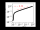
\includegraphics[width=0.4\textwidth]{figures/1_tuning_curves_SI}
\caption{Distribution of $K^{ai}$ is drawn from a a power law distribution with exponent $\alpha = 0.35$ as found in ~\cite{si2017invariances}.}
\label{fig:SI_power_law}
\end{figure}
\fi

\begin{figure}
\centering
\includegraphics[width=0.6\textwidth]{figures/2_coding_representation_SI}
\caption{Front-end adaptive feedback preserves information capacity of the ORN sensing repertoire. Mutual information between signal $\mathbf s(t)=\mathbf s_A(t)+\mathbf s_B(t)$ and response $\mathbf r(t)$ is calculated at various points in time $t$ for an odor environment consisting of two step odors, A and B. 
\textbf{A} Odor A, with concentration $\mathbf s_A(t)$, turns on at time $t_A$ and a odor B, with concentration $\mathbf s_B(t)$, turns on at some later time $t_B$. Both odors have similar intensities $\sim s_0$ and similar molecular complexity ($k = 4$). 
\textbf{B} Mutual information as a function of $s_0$ for the non-adaptive system, respectively, at different time points after $t_A$, corresponding to the dots in A. The mutual information carried by distinct ORNs is represented by the shaded region; their average is plotted by the heavy line. In the non-adaptive system, the mutual information peaks in the regime of high sensitivity after the arrival of odor A (purple, blue), and shifts leftward with the onset of odor B (teal, green). The leftward shifts occurs since stronger signals are more prone to response saturation (compromising information transfer) as odor B arrives. 
\textbf{C} Same as B, now for the adaptive system. The MI mimics the non-adaptive case at the onset of odor A, before adaptation has kicked in (purple). As the system adapts and responses decrease toward baseline, previously saturating signal intensities now cross the regime of maximal sensitivity, which therefore shifts rightward to higher $s_0$ (dark blue). Much later, but before the arrival of odor B, the ORNs that responded now fire at a similar  adapted firing rate $\sim 30$ Hz, irrespective of odor identity, so the mutual information drops to zero. However, having now adjusted its sensitivity to the presence of odor A, the system can respond appropriately to odor B: the MI at $t_B$ is nearly 6 bits across decades of concentration immediately following $t_B$ (green). 
}
\label{fig:SI_MI}
\end{figure}


\begin{figure}
\centering
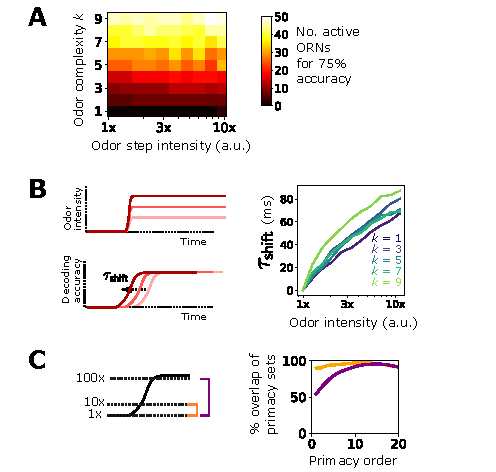
\includegraphics[width=0.7\textwidth]{figures/4_primacy_coding_SI}
\caption{Additional results pertaining to the primacy coding hypothesis. 
\textbf{A} Percent of active ORNs required for 75\% accuracy of a steep sigmoidal odor step, as a function of odor step intensity and odor complexity. For low complexities, a primacy set of fewer ORNs may be sufficient to decode the full odor signal; for higher complexities, the entire ORN repertoire is required.
\textbf{B} In the primacy coding hypothesis, the primacy set is realized sooner for stronger odor signals, so odors are decoded earlier in time, resulting in a perceptual time shift with increasing odor concentration ~\cite{primacy_coding}. We also find this shift in our compressed sensing decoding framework (right plot), which rises monotonically with step height for various odor complexities, in agreement with primacy coding.
\textbf{C} The consistency of a primacy code across changes in background odor concentration, in a system with Weber Law adaptation. We calculate the primacy set for odor A (step odor; black) in the presence of either a weak, medium, or strong background (dotted lines; 1x, 10x, 100x a.u.), assuming the system has adapted its response to the background as described in the main text. Averaged across odor A identities, primacy sets for odor A when in the 1x background are nearly identical to those when odor A is in the 10x background (right plot; yellow). The same holds true when comparing the 1x and 100x backgrounds, for sufficiently large primacy order, above 8 or so right plot; purple). This indicates that Weber Law adaptation preserves primacy codes across disparate environmental conditions.
}
\label{fig:SI_primacy}
\end{figure}

\begin{figure}
    \centering
    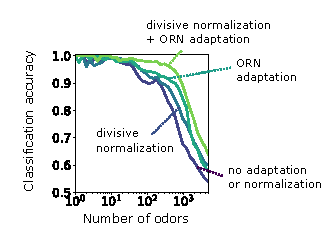
\includegraphics[width=0.6\textwidth]{figures/5_downstream_SI.pdf}
    \caption{Accuracy of binary classification  by odor valence, for odors whose concentrations span a narrow range of concentrations (1 order of magnitude). Accuracy is plotted as a function of the number of distinct odor identities classified by the trained network, in systems with only ORN adaptation, only divisive normalization, both or neither. Decoding gains conferred by divisive normalization and/or ORN adaptation are much smaller than when odors span a much larger range of concentrations, as shown in the main text.}
    \label{fig:SI_downstream}
\end{figure}



\begin{figure}
\centering
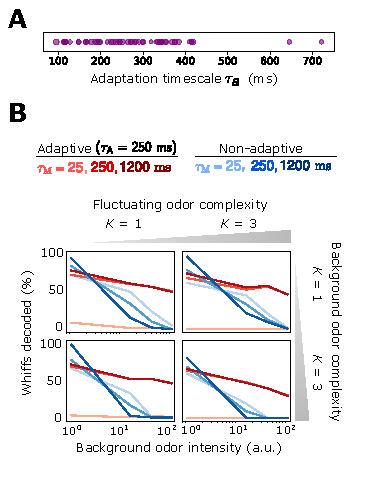
\includegraphics[width=0.6\textwidth]{figures/temporal_broad_tA.pdf}
\caption{Decoding accuracy for system with broader distribution of adaptive timescales $\tau$.
\textbf{A} Distribution of timescales for all ORNs $a$ (purple dots). Here, $\tau_a \sim = 10^X$ where $\tau = 250$ ms as in the main text and $X \sim \mathcal N(0, 0.2)$. 
\textbf{B}  Individual plots show the percent of accurately decoded odor whiffs (same fluctuating odor signal used in the main text) as a function of background odor intensity, for the non-adaptive (blue) and adaptive (red) systems, for different $\tau_M$ (line shades). Plots are arrayed by the complexity of the naturalistic signal (column-wise) and the complexity of the background odor (row-wise).
}
\label{fig:SI_broad_tA}
\end{figure}



\begin{figure}
\centering
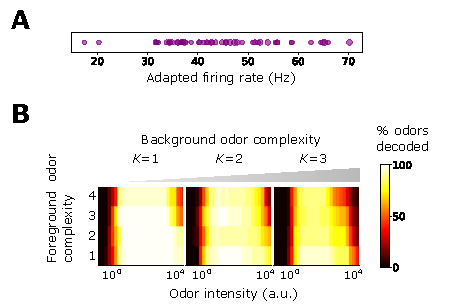
\includegraphics[width=0.8\textwidth]{figures/broad_A0}
\caption{Benefits conferred by Weber-Fechner adaptation remain for a broader distribution of baseline firing rates $A_{a0}$, now assumed to be ORN-dependent and chosen from a normal distribution.
\textbf{A} Distribution of $A_{a0}$.
\textbf{B} Decoding accuracy of foreground odors in the presence of background odors.}
\label{fig:SI_broad_A0}
\end{figure}


\begin{figure}
\centering
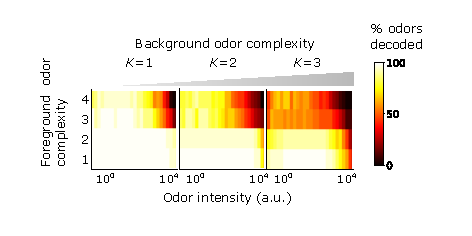
\includegraphics[width=0.8\textwidth]{figures/2_binding_sites}
\caption{Benefits conferred by Weber-Fechner adaptation remain for 2 binding sites per receptor. This might conceivably occur in insect olfactory receptors, heterotetramers consisting of 4 Orco/Or subunits that gate a central ion channel pathway~\cite{orco_structure}. Plotted is the decoding accuracy of foreground odors in the presence of background odors.
}
\label{fig:SI_mult_binding}
\end{figure}


\begin{figure}
\centering
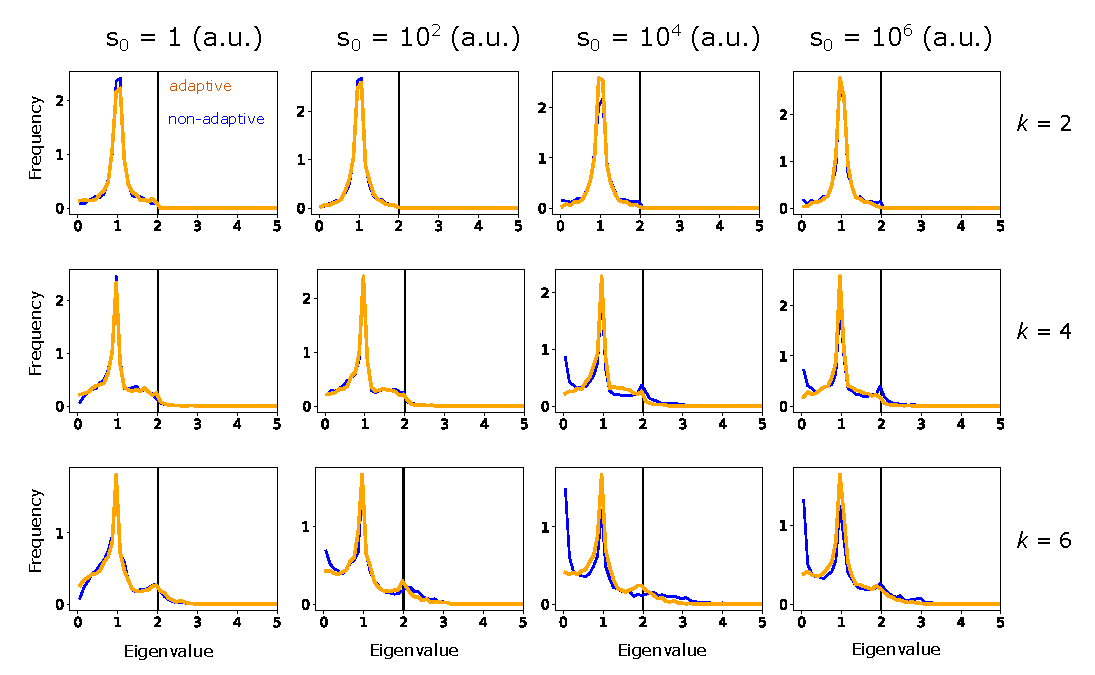
\includegraphics[width=0.95\textwidth]{figures/HIT_eigs}
\caption{Eigenvalue distribution of $\mathbf{A}_{\mathbf x_n}^T\mathbf{A}_{\mathbf x_n}$, where $\mathbf{A}_{\mathbf x_n}$ is a $m \times k$ submatrix of the  column-normalized linearized ORN response matrix $\mathbf{A}$, evaluated at the linearization point $\mathbf x_n$. Note that $\mathbf x_n$ is $k$-sparse, but its components do not necessarily align with the $k$ columns chosen for the sub-matrix. Eigenvalues are calculated for the adaptive (orange) and non-adaptive (blue) systems, for 1000 randomly chosen linearization points $\mathbf x_n$ and submatrices. Plots are arranged for various odor sparsities (by row) and odor intensities (by column). The restricted isometry property is satisfied when the eigenvalues lie between 0 and 2 (black vertical line), and is more strongly satisfied the more centered the distribution is around unity. The increase in near-zero eigenvalues for the non-adaptive system at higher odor complexities and intensities (lower right plots) indicates the weaker fulfillment of the restricted isometry property for thhse signals, and leads to higher probability of failure in compressed sensing signal reconstruction.
}
\label{fig:SI_HIT_eigs}
\end{figure}


\begin{figure}
\centering
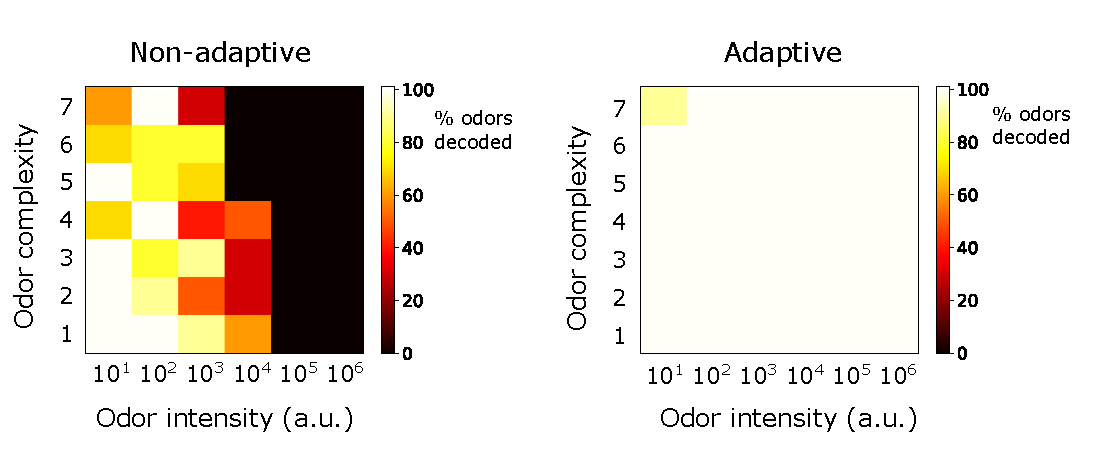
\includegraphics[width=0.8\textwidth]{figures/HIT_est}
\caption{Decoding of odor signals (no background odors) using the IHT algorithm~\cite{IHT, nonlin_CS} qualitatively reproduces the results from the main text, which used traditional CS with background linearization. In the adaptive case, IHT actually exhibits superior accuracy to traditional CS, though IHT demands more compute time. The results here show odor decoding accuracy for sparse odor signals of given complexity and intensity, averaged over 10 distinct identities. Odors are considered accurately decoded if the $K$ sparse components are estimated within 25\% and the components not in the mixture are estimated below 10\% of $s_0$. The iterative algorithm was initialized at $ \hat{ \mathbf x} = \mathbf 0$ and run forward until $ \hat{ \mathbf x}$ was stationary, or 10000 iterations were reached. Step size $\mu$ in Eq.~\ref{eq:IHT_NL} was set to $s_0/20$. At each step, the linearized response ($\mathbf{A}_{\mathbf x_n}$ in Eq.~\ref{eq:IHT_NL}) was evaluated at the result of the previous iteration. IHT also requires an assumption on the number of components in the mixture (which defines  $H_K(\cdot )$ in Eq.~\ref{eq:IHT_NL}); here, that was set to twice the actual sparsity of true signal. 
}
\label{fig:SI_IHT_est}
\end{figure}


\begin{figure}
\centering
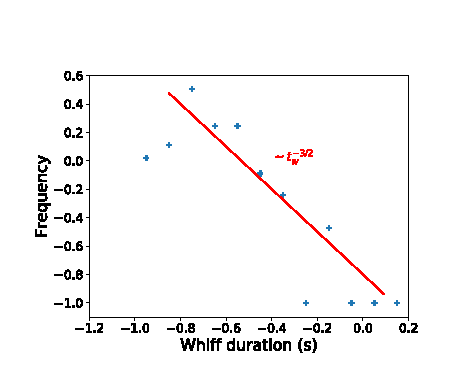
\includegraphics[width=0.6\textwidth]{figures/3_decoding_temporal_SI}
\caption{Distribution of whiff durations in naturalistic stimulus, compared to the theoretical prediction~\cite{celani}.
}
\end{figure}



\iffalse
\begin{table}\centering
\caption{This is a table}

\begin{tabular}{lrrr}
Species & CBS & CV & G3 \\
\midrule
1. Acetaldehyde & 0.0 & 0.0 & 0.0 \\
2. Vinyl alcohol & 9.1 & 9.6 & 13.5 \\
3. Hydroxyethylidene & 50.8 & 51.2 & 54.0\\
\bottomrule
\end{tabular}
\end{table}
\fi 

%%% Add this line AFTER all your figures and tables
\FloatBarrier

\iffalse
\movie{Type caption for the movie here.}

\movie{Type caption for the other movie here. Adding longer text to show what happens, to decide on alignment and/or indentations.}

\movie{A third movie, just for kicks.}

\dataset{dataset_one.txt}{Type or paste caption here.}

\dataset{dataset_two.txt}{Type or paste caption here. Adding longer text to show what happens, to decide on alignment and/or indentations for multi-line or paragraph captions.}
\fi

\bibliography{bibliography}

\end{document}